\chapter{Desenvolvimento do Sistema Supervisório}

\section{Requisitos do Sistema}

Para a escolha da tecnologia empregada, foram levantados os seguintes requisitos do sistema:
\begin{itemize}
	\item Deve ser gratuito para o desenvolvimento, simples e de código aberto no intuito de permitir análise por partes de interessados e facilitar melhorias e expansões;
	\item Deve ser capaz de plotar gráficos em tempo real, advindos de no mínimo porta serial. Opcionalmente pode ser compatível com arquivos nos formatos .csv, .tsv, .xls, e .xlsx, ou permitir modelagem direta no software, por funções de transferência
	\item O software deve rodar no sistema operacional windows (mínimo Windows 7)
\end{itemize}

\section{Seleção das Tecnologias}

Pelo primeiro requisito, em relação à gratuidade da tecnologia, pensou-se primeiramente em utilizar plataformas abertas para sistemas supervisórios, como o ScadaBR ou a versão demo do Elipse E3. Já houveram trabalhos, inclusive, utilizando a primeira tecnologia (referenciados na bibliografia deste documento).

Como atestado em \cite{Moraes2016}, o ScadaBR é construído em um servidor web, utilizando geralmente o Apache TomCat (como servidor web). Assim, julgou-se necessário um certo período para acostumar-se com a sua programação, além de um conhecimento em redes para configuração da comunicação cliente-servidor.

Quanto à versão demo do Elipse E3, apesar do autor já possuir certo domínio da ferramenta, se trata de uma versão muito limitada. Segundo sua base de conhecimento, \cite{Elipse2019}, a versão demo permite somente até 20 tags de dados e a aplicação roda por um máximo de 2 horas, tendo que ser reiniciada manualmente após este período. Finalmente, não se sabe as implicações legislativas em utilizar o software para trabalhos acadêmicos, nem sua utilização contínua no âmbito da universidade, mesmo se tratando de uma versão de demonstração.

Por cumprir todos os requisitos, e por ser considerado um método inovador, foi decidido construir um sistema SCADA em Python. Desta maneira, o código-fonte da aplicação seria aberto, sua programação não exigiria grande esforço por parte do programador, e este trabalho contribuiria na difusão da implementação de softwares gratuitos e open source no meio acadêmico. Além disto, Python é uma linguagem contemporânea, tendendo a acompanhar o avanço tecnológico. Desta forma o sistema desenvolvido seria compatível com uma vasta gama de tecnologias atuais e futuras.

\subsection{Seleção das bibliotecas}

Como já mencionado, a linguagem Python possui inúmeras bibliotecas, para os mais variados fins. No decorrer da criação do sistema, foram utilizadas as seguintes bibliotecas no Quadro \ref{qdr_used_libs}.

\begin{quadro}
	\centering
	\begin{tabular}{|m{5em}|m{25em}|}
		\hline
		Biblioteca & Descrição \\
		\hline
		PyQt5 & Usada para a construção de GUIs, contém diversos objetos úteis como botões, caixas de texto e rótulos. Também trata do posicionamento e direção destes objeto nas janelas principal e periféricas \\
		\hline
		matplotlib & Contém ferramentas que permitem a plotagem e design de gráficos variados, inclusive com objetos backend que fazem uma ponte com GUIs construídas com PyQt5 \\
		\hline
		numpy & Biblioteca que lida com operações matriciais e cálculos avançados, com muitas funcionalidades similares ao MatLab. Também é capaz de gerar números aleatórios, que são úteis no teste do programa \\
		\hline
		pyserial & Permite a conexão com dispositivos externos pela porta serial e contém funções de escrita e leitura desta porta \\
		\hline
		python-control & Possibilita a criação de sistemas descritos em funções de transferência e espaço de estados, além de gerar a resposta simuladas para alguns formatos comuns de entradas, como degrau e impulso \\
		\hline
		pickle & Responsável pera serialização de objetos utilizados no código e armazenamento dos mesmos em um arquivo à parte. Lida também com a leitura e decodificação de objetos serializados \\
		\hline
	\end{tabular}
	\caption{Bibliotecas Python utilizadas no desenvolvimento do supervisório didático}
	\label{qdr_used_libs}
\end{quadro}

\section{Criando a interface gráfica}

A biblioteca PyQt funciona como uma linguagem orientada a objetos. Assim, esta arquitetura foi adotada no desenvolvimento da ferramenta. Foi utilizado uma folha de script que agrupasse a maior parte das classes implementadas, o form\_objects.py, e outro script principal, main.py que inicia a execução do programa. Um terceiro script, realtime\_objects.py, contempla objetos que rodam em tempo real e espera-se que futuros usuários também editem o código contido, por motivos explanados posteriormente neste documento.

No que concerne a interface gráfica do supervisório, imaginou-se um layout simplista. A aplicação conteria uma área para plotagem de gráficos, uma lista das séries de dados incluídas no programa pelos diversos métodos possíveis, e uma área para incluir séries novas. Os detalhes destes Widgets são listados abaixo, e sua disposição mostradas na Figura \ref{img_gui_macro}:

\begin{itemize}
	\item \emph{PlotManager}:representaria uma área de rolagem (QScrollArea) que conteria várias representações gráficas das séries de dados salvos na aplicação, com um pequeno preview destes dados, e botões para sua plotagem, edição e exclusão da série.
	\item \emph{MainPlotArea}: utiliza um objeto \emph{FigureCanvas}, da lib matplotlib, para plotagem detalhada das séries selecionadas na lista de séries. O eixo y seria adimensional, dependendo da variável medida e observada, e o eixo x representaria o tempo.
	\item \emph{DatasetConfig}: tem como Widget principal um seletor com abas (\emph{QTabWidget}), que permitiria a inclusão de séries de dados novas no programa, pelas fontes já mencionadas, sendo cada aba responsável pelas diferentes métodos (serial, arquivo, função de transferência, etc)
	\item \emph{SCADADialog}: se trata realmente de uma tela de supervisão, com uma área de plotagem atualizada em tempo real. Funciona somente quando os dados são importados por porta serial.
\end{itemize}

\begin{figure}[hbt]
	\centering
	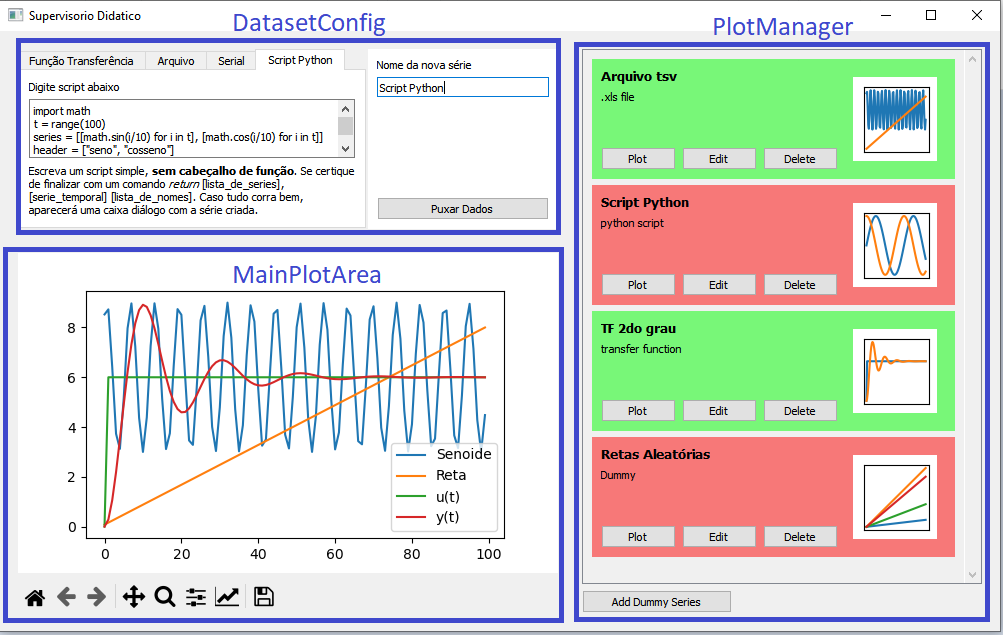
\includegraphics[width=\textwidth]{GUI_macro}
	\caption{Supervisório didático e seus objetos principais}
	\label{img_gui_macro}
\end{figure}

Além dos Widgets supracitados, para simplificar o código e troná-lo mais prático, foi criado um objeto abstrato \emph{SeriesObject}. Ele armazena um agrupamento de série de dados que compartilham um mesmo eixo de tempo. Desta forma, foi mais fácil manipular as referências das séries pelo programa.

\section{\emph{Dataset Config}}

A principal função deste objeto é de interface da aplicação com outros dispositivos ou programas, com a finalidade de puxar séries de dados destas fontes. A segunda função é de formatar estas séries, atribuindo a elas um nome e um cabeçalho, além de definir que legenda aparece no gráfico principal quando a série for plotada.

Na fase de idealização do software, levantou-se possíveis meios para adicionar séries de dados novas no programa. Como se trata de um sistema supervisório, deve haver uma funcionalidade que permita o recebimento de dados externos, no mínimo por comunicação serial, bastante utilizada por controladores didáticos como Arduino e Raspberry Pi. Como adicionais,, seria útil também a importação de séries por arquivos \emph{.xls} ou \emph{.xlsx}. Por último, caso o usuário deseje utilizar funcionalidades não ofertadas pelo software didático, ele pode escrever seu próprio script Python e levar os resultados para o programa.

Na engenharia de Controle e Automação, é comum a prática de modelar um processa antes de observar seu comportamento empírico. Visto isso, o programa deveria oferecer uma maneira simples de simular processos diversos e plotá-los em contraste com o sistema real, proveniente do controlador. Logo, foi incluída biblioteca que simulasse as resposta de funções de transferência, por padrão a uma entrada degrau, e fornecidos os meios para que o usuário encadeie em série variadas funções, de parâmetros quaisquer, pelo objeto \emph{TransferFunctionConfig}.

Resumindo, existem quatro maneiras de importar ou gerar uma série de dados no software desenvolvido:

\begin{enumerate}
	\item \textbf{Por arquivo}, nos formatos \emph{csv} (Comma Separated Values), \emph{tsv} (Tab Separated Values), \emph{xls} (antigo arquivo Excel), \emph{xlsx} (arquivo Excel);
	\item \textbf{Por função de transferência}, informando o numerador e denominador de cada função, criadas em série e submetidas a uma entrada do tipo degrau, de valor definido pelo usuário;
	\item \textbf{Por comunicação serial}, configurando alguns parâmetros (porta, baud rate e tempo para timeout), separando cada valor enviado pelo dispositivo por uma tabulação e linhas por quebras de linha;
	\item \textbf{Por script Python}, escrevendo um código python funcional e retornando os valores das séries na ordem correta (lista dos valores das séries, série de valores de tempo, lista de nomes das séries, nesta ordem)
\end{enumerate}

Caso não haja problemas na importação e as condições de formatação para cada método de entrada forem satisfeitas, o programa abrirá uma caixa diálogo (\emph{QtWidgets.QDialog}) idêntica à da Figura \ref{img_edit_series_dialog} com uma preview dos dados e uma tabela com os valores numéricos. Através dele é possível editar cada valor separadamente, o nome da série e o cabeçalho.

\begin{figure}[hbt]
	\centering
	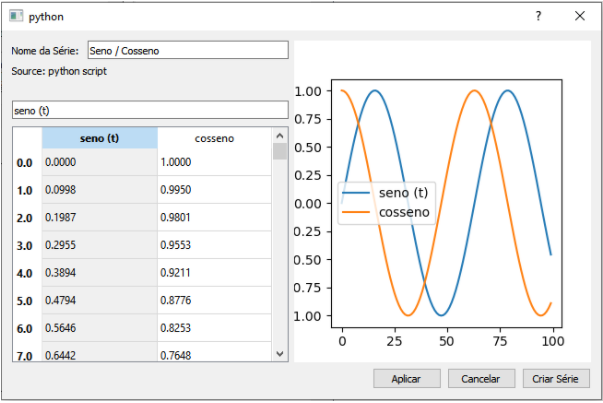
\includegraphics[width=\textwidth]{edit_series_dialog}
	\caption{\emph{ModelSeriesDialog}: Caixa diálogo para edição dos eixos e título das séries}
	\label{img_edit_series_dialog}
\end{figure}

A caixa diálogo contém um Widget bastante importante para a aplicação: o \emph{FigureCanvas}, proveniente de um módulo da biblioteca matplotlib, que funciona como um plugin para o PyQt. Apesar dele não ser um Widget do PyQt, ele contém, se não todos, uma boa parte de seus módulos e é tratado como tal para fins de posicionamento, geometria e inclusão nos layouts de tela. O \emph{FigureCanvas} faz uma interface com o objeto \emph{Figure}, responsável pela plotagem de gráficos de linhas, barras, etc, e permite que ele seja incluído numa GUI construída em PyQt.

O objeto \emph{Figure}, por sua vez, é bem similar ao objeto de mesmo nome no MATLab\textsuperscript{\tiny \textregistered}, aceitando métodos como \emph{plot()}, emph{add\_subplot()} e \emph{clear()}. Sua documentação completa, juntamente com a de outros objetos relevantes consta no site da biblioteca \href{https://matplotlib.org/}{matplotlib}. Quando embutido numa GUI por um \emph{FigureCanvas}, após a plotagem de gráficos e de formatações gerais, o segundo deve chamar o método \emph{draw()} para que seja atualizada a imagem.

%\textcolor{red}{Devo Focar no algoritmo de cada tipo de importação??}

\section{\emph{PlotManager}}

No lado direito da aplicação, se encontra uma lista das séries carregadas. Dado o espaço limitado, faz-se necessária uma área de rolagem. Assim, foi criado um objeto \emph{GraphicPlotList} que implementa esta área ao herdar de \emph{QtWidgets.QScrollArea}. Também existia originalmente um botão que criasse uma série de até 4 retas com inclinações aleatórias, para fins de teste.

Quando uma série nova é criada pelo \emph{DatasetConfig}, ela fica armazenada em um objeto \emph{SeriesObject}, que é representado graficamente na lista de séries \emph{GraphicPlotList} por um outro objeto \emph{GraphicPlotConfig} (Figura \ref{img_graphic_plot_config}).

\begin{figure}[hbt]
	\centering
	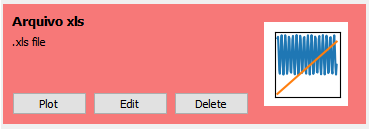
\includegraphics{graphic_plot_config}
	\caption{\emph{GraphicPlotConfig} não plotado em \emph{MainPlotArea}}
	\label{img_graphic_plot_config}
\end{figure}

A principal função deste objeto é identificar pelo nome e fonte a série que contém, e coordenar quando esta série deve ser plotada na área principal \emph{MainPlotArea}, além de permitir sua edição ou deleção. Contribuindo com a identificação dos dados, foi incluída uma visualização simples das séries, o que torna o visual estético. A cor de fundo do \emph{GraphicPlotConfig} alterna entre verde e vermelho, indicando se as séries contidas foram plotada ou não. Ao clicar no botão “Edit”, uma caixa diálogo idêntica à de incluir uma série nova aparece permitindo que o usuário edite seus valores, cabeçalho e nome.

Em PyQt, os objetos de uma GUI são “pintados” na tela por um objeto \emph{QtGui.QPainter}, de acordo com sua área, e paleta de cores. A primeira informação depende de alguns parâmetros, como o layout no qual ele está inserido ou sua política de tamanho (QSizePolicy). Isto ocorre no método \emph{paintEvent(event)}, chamado automaticamente quando o objeto é reposicionado ou quando sua aparência deve ser atualizada (cada caractere novo digitado numa caixa de texto, por exemplo).

Essa dinâmica torna necessário que o método seja sobrecarregado quando o programador deseje customizar a aparência de um botão ou o seu plano de fundo. A desvantagem é que, por sobrecarregar o método que pinta o objeto na interface, o objeto deve ser repintado manualmente. No caso de um botão, por exemplo, no mínimo o método \emph{drawRectangle()} e \emph{drawText()} deve ser invocado. Assim, quanto mais detalhado for um objeto, mais complicado se torna alterar suas cores e formatos internos. Existem maneiras que contornam a necessidade de criar um novo objeto e sobrescrever o método paintEvent, utilizando as chamadas stylesheets. Porém, para este trabalho, julgou-se mais simples a primeira opção, pelo fato dos objetos customizados possuírem um design pouco complexo.

O objeto \emph{GraphicPlotConfig}, por alternar suas cores de fundo, teve seu evento de "pintura" sobrecarregado. Como sua tela de fundo é representada apenas por um retângulo, sua implementação não foi muito dificultosa.

\section{\emph{MainPlotArea}}

Se tratando de análises de sistemas, a visualização dos dados é essencial. No canto inferior esquerdo da GUI, existe uma área de plotagem, implementada por um objeto \emph{FigureCanvas} (Figura \ref{img_main_plot_area}. Abaixo dele, uma faixa de ferramentas (\emph{NavigationToolbar2QT}) permite que o usuário edite algumas propriedades do gráfico plotado, aproxime ou distancie a imagem e, principalmente, salve a figura em formato de imagem. Na lista de séries à direita, ao clicar no botão “Plot”, a série associada serão desenhadas no Canvas, com legenda.

\begin{figure}[htb]
	\centering
	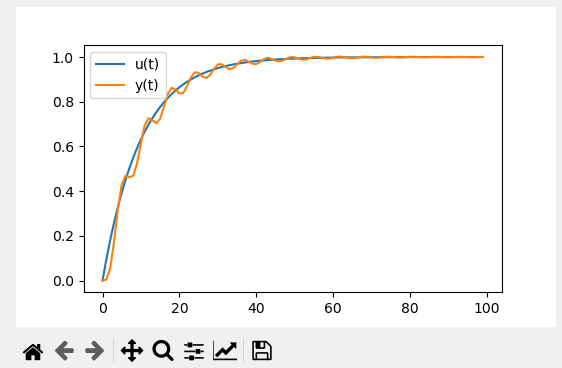
\includegraphics[width=0.8\textwidth]{main_plot_area}
	\caption{\emph{MainPlotArea}}
	\label{img_main_plot_area}
\end{figure}

\section{\emph{SCADADialog}}

Um sistema supervisório, como o apresentado neste documento, monitora dados de controladores geralmente industriais em tempo real. Por se tratar de um software didático, pensou-se em inclui no programa um suporte para futuras comunicações com um Arduíno ou qualquer outro microcontrolador ou até mesmo dispositivos que permitam comunicação serial. Assim, configurados os parâmetros de comunicação (\emph{baud rate}, nome da porta e tempo de timeout), o usuário pode plotar dados enviados por um controlador em tempo real, desde que os mesmos estejam no formato esperado: tabulações para separar diferentes séries de dados e quebras de linhas para finalizar um registro.

Ao importar dados por fonte serial no \emph{DatasetConfig}, sugere-se sempre testar a comunicação antes de clicar no botão “Puxar dados”. quando o mesmo é clicado, uma caixa diálogo \emph{DialogHeader} é aberta, para que o usuário edite os nomes das variáveis recebidas via serial. A primeira série é sempre o tempo, e o dispositivo conectado \textbf{deve} obedecer esta ordem. Ao clicar em OK nesta caixa, a comunicação com a porta serial será iniciada e uma janela de monitoramento surgirá, caso não tenha ocorrido nenhum erro de comunicação.

%Vale a pena colocar referencia nestes trechos
O código por trás da comunicação com periféricos implementa duas threads da biblioteca nativa emph{\_thread} do Python. Threads são trechos de código que rodam simultaneamente em um mesmo processo pai. Por conta disso, ao utilizar esta estrutura, alguns cuidados devem ser tomados pelo programador, no que se refere a acesso compartilhado à memória. Como não há controle de execução de cada thread separadamente, bugs podem ocorrer caso mais de um processo acesse e modifique o mesmo objeto ou variável simultaneamente.

Para contornar este problema, existem algumas estruturas que controlam o acesso de memória em programas que implementam threads, como monitores e semáforos. O último é, talvez, o mais trivial. Um semáforo possui dois estados: aberto ou fechado. Quando uma thread toma controle de um objeto no código, o semáforo é fechado, impedindo que outras threads façam o mesmo, até que o objeto seja liberado e o semáforo reaberto. Para Python, existem bibliotecas que implementam estruturas de controle, como a \emph{asyncio}, porém, por ser uma estrutura simples e não utilizada mais que algumas vezes no código-fonte deste trabalho, uma variável booleana bastou.

Após a conexão bem sucedida com o dispositivo, o programa escreve uma mensagem na porta serial (“go”, por padrão) e inicia suas duas threads, uma para ler dados da porta, e outra para atualizar o Canvas da caixa diálogo \emph{SCADADialog}. Esta separação se fez necessária pois o método do Canvas que o atualiza (emph{draw()}) é considerado custoso, e poderia travar a aplicação se fosse executada repetidas vezes. Outro motivo para implementação das threads é exemplificar a estudantes do código uma implementação simples de paralelismo, o que pode ser bastante util e que não é abordadas nos cursos tradicionais de Engenharia (excetuando computação).

Cada uma das threads tem um tempo de repetição, que define a periodicidade que elas executam suas instruções. O padrão definido foi de 0,1 segundos para ler dados da porta serial, e 1 segundo para atualizar o gráfico com os valores lidos. Quando a leitura da porta ocorre, os valores são armazenados em uma lista chamada emph{to\_be\_plotted}. Quando o gráfico é atualizado, os valores desta lista são movidos para outra, chamada emph{plotted}, que por sua vez é plotada, e o gráfico atualizado. A manipulação compartilhada da lista to\_be\_plotted justifica o emprego de um semáforo, pois uma thread escreve e outra lê.

Como já mencionado, o programa espera que os dados recebidos sejam espaçados por tabulações, separando diferentes variáveis, e quebras de linhas, separando diferentes leituras ao longo do tempo de execução. O primeiro valor lido sempre é considerado o tempo, e deve vir do dispositivo conectado, pois o mesmo é quem dita o andamento do processo controlado. Caso o número de variáveis numa mesma linha lida seja diferente do configurado no objeto DatasetConfig, o programa considerará que houve um erro e toda a linha de dados será ignorada.

A figura \ref{img_esquema_serial} esquematiza a execução do código de monitoramento serial:

\begin{figure}[hbt]
	\centering
	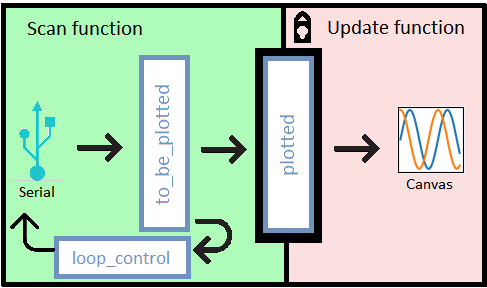
\includegraphics{esquema_serial}
	\caption{Esquema de leitura serial no supervisório didático}
	\label{img_esquema_serial}
\end{figure}

Para que o programa possa ser de fato implementado em aulas do curso, foi adicionada a possibilidade de envio de dados ao controlador a cada leitura da porta serial. Isto seria uma analogia a um controlador que atuasse num processo físico, medido por um dispositivo conectado. Devido à popularidade do microcontrolador Arduino, a implementação da rotina de controle foi projetada similarmente à sua programação. A rotina é feita em duas etapas, uma na função \emph{setup\_control}, chamada logo após uma conexão bem-sucedida, uma única vez, e outra na função \emph{loop\_control}, chamada logo após cada leitura da porta serial.

Numa aplicação de controle PID, por exemplo, a primeira função realizaria sua sintonia, enquanto que a segunda receberia como parâmetro a última linha lida da porta, calcularia a resposta do controlador PID, e a escreveria de volta. Obviamente, o dispositivo conectado deve ser programado para receber esta informação, o que requer certo conhecimento do usuário, tanto de Python como do dispositivo utilizado. Felizmente, códigos de exemplo se encontram disponíveis neste documento.

Durante o monitoramento e registro dos valores trazidos via serial, o gráfico irá atualizar numa janela de 20 segundos, contando do maior tempo registrado para trás. Isto se justifica no comportamento dinâmico da maioria dos sistemas, que atinge valores por vezes maiores que os estacionários. Esta medida impede que a escala do gráfico fique prejudicada, e variações pequenas relativas a um comportamento estacionário não sejam bem percebidas. O usuário pode, de todo modo, em tempo de execução clicar nos botões “Parar” e “Criar Série”, salvar as séries de dados lidas e plotá-las no objeto MainPlotArea, visualizando todo seu comportamento histórico.

\section{Salvamento Automático de Séries}

Durante a realização do caso de teste, descrito posteriormente neste documento, percebeu-se que no decorrer da análise de processos muitos ajustes são realizados, seja na função de controle da aplicação ou no controlador. Quando o script Pyhton é iniciado, uma cópia dele é criada e compilada, tornando impossível que alterações no script original em tempo de execução tenham influências no sistema. Por isso, o usuário tem que fechar o supervisório didático sempre que desejar alterar as funções \emph{setup\_control()} e \emph{loop\_control()}, o que resultaria na perda das séries já salvas pelo programa.

Para amenizar este problema, foi incluída uma funcionalidade de salvamento automático na aplicação. Uma das bibliotecas nativas do Python, o \emph{Pickle}, permite que um objeto ou variável do programa seja serializada em formato de arquivo, e salva em um diretório no computador. Isto ocorre através do comando \emph{pickle.dump()} Desta forma, o arquivo pode ser restaurado (\emph{pickle.load()}) e reincorporado ao código com os mesmos valores de atributos que possuía quando foi serializado.

Sempre que uma série é incluída, editada ou deletada, o arquivo "autosave.dat" é sobrescrito com a lista de séries da sessão (\emph{listSeries}). Em contrapartida, quando o objeto \emph{PlotManager} é inicializado, o arquivo "autosave.dat" é aberto e a lista de séries lá salva é restaurada.

\section{Diagrama de Relações entre Objetos}

A Figura \ref{img_diagrama_objetos} ilustra todos os objetos utilizados na construção do software, suas relações e principais métodos.

\begin{figure}[hbt]
	\centering
	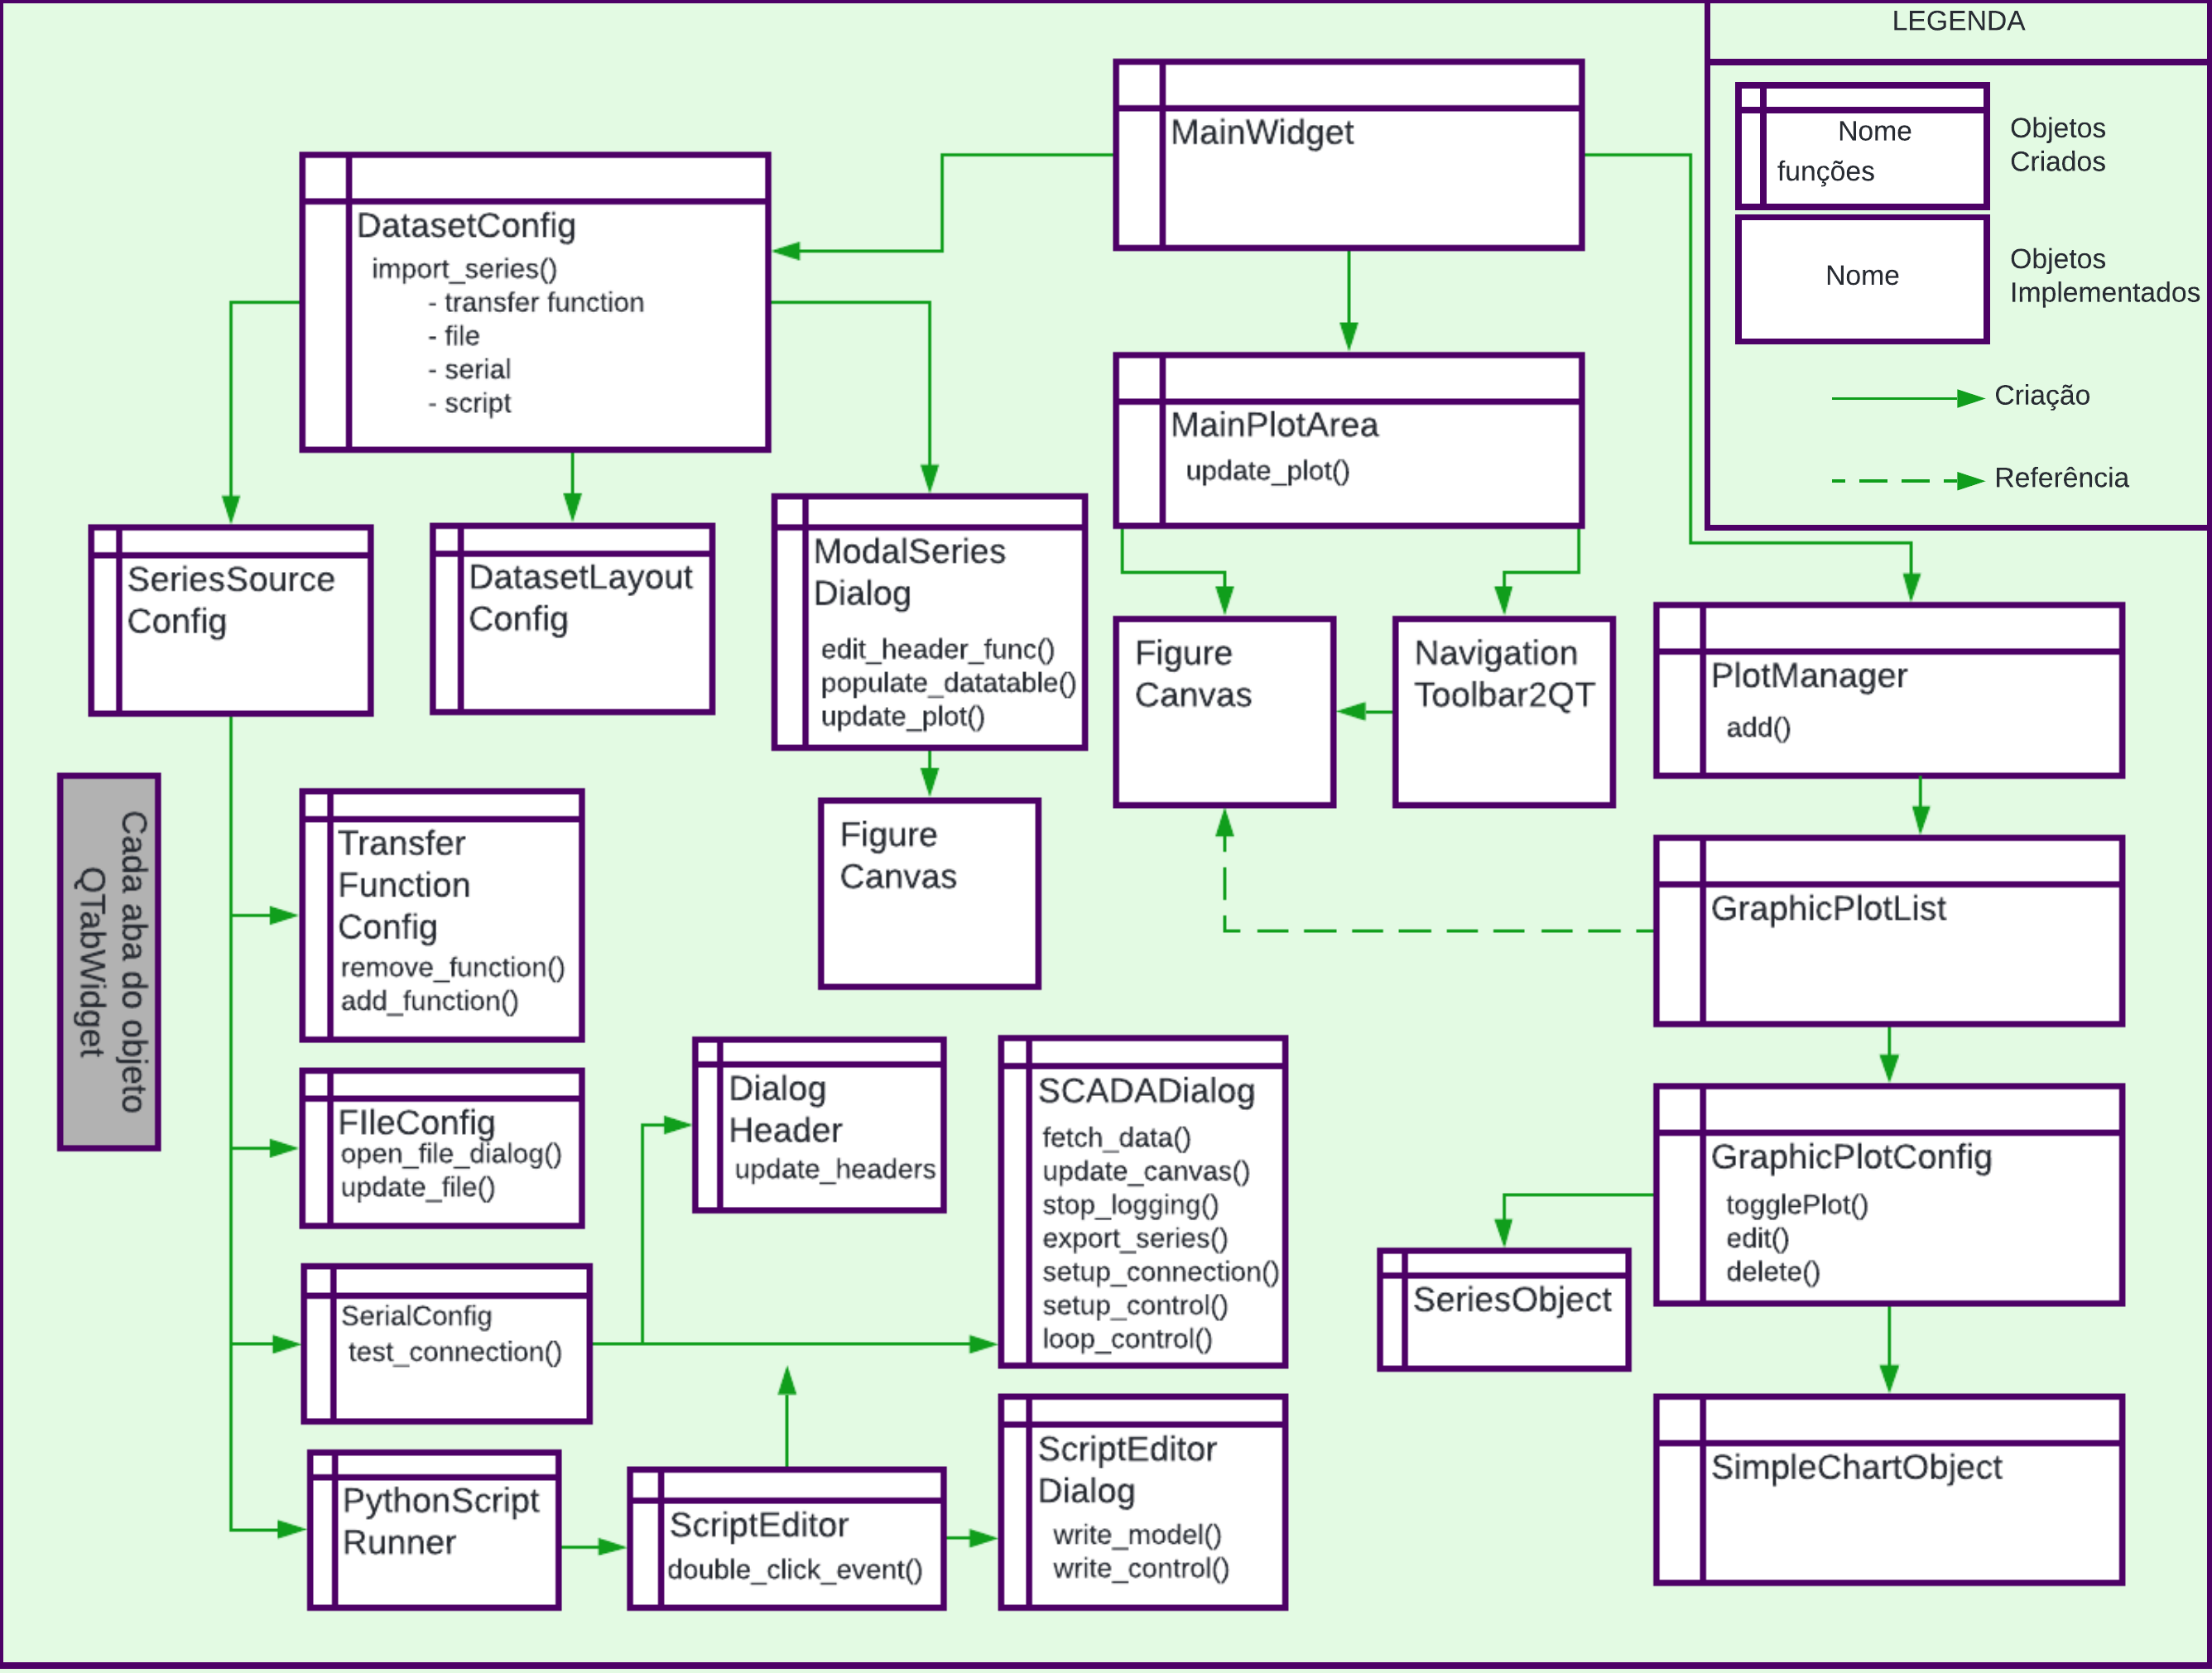
\includegraphics[angle=90, width=\textwidth]{diagrama_objetos}
	\caption{Diagrama de relações entre os objetos empregados e funções principais}
	\label{img_diagrama_objetos}
\end{figure}